\chapter{Experimental Results and Analysis of CCTVVS}

In analysis of a process, experiments are commonly used to evaluate the inputs
to the process which most times define the output of the process. They also
help pinpoint the appropriate and thus target inputs to achieve a desired
result. The output of the video summariser is compared with the expected output
to verify the correctness of the system. There are several metrics for
comparison. Analyzing the experimental output is verifying whether the
evaluation metrics are satisfied. This chapter discusses the performance
characteristics of the system.

\section{Evaluation Metric}

Evaluation metrics are the criteria for testing different algorithms. The
behavior of the algorithms or techniques can be determined using these metrics.
In this project, there are not many concrete objective methods for testing the
summary, and some metrics are subjective as well. The outputs that are
obtained from the different inputs given to the summariser are compared with
the expected output to check whether the metrics are satisfied.

\section{Experimental Dataset}

Sample video clips in different urban areas with sparse motion and activity were
collected, with only 1-2 events occurring once every few seconds. These clips
were used for developing and testing the algorithm.

Figure~\ref{img:sample-input} shows some frames from one of our experimental
videos. Only 1-2 events are seen occurring at any point of time. People and
bikes are the objects that are seen.

\begin{figure}[!htb]
    \minipage{0.32\textwidth}
        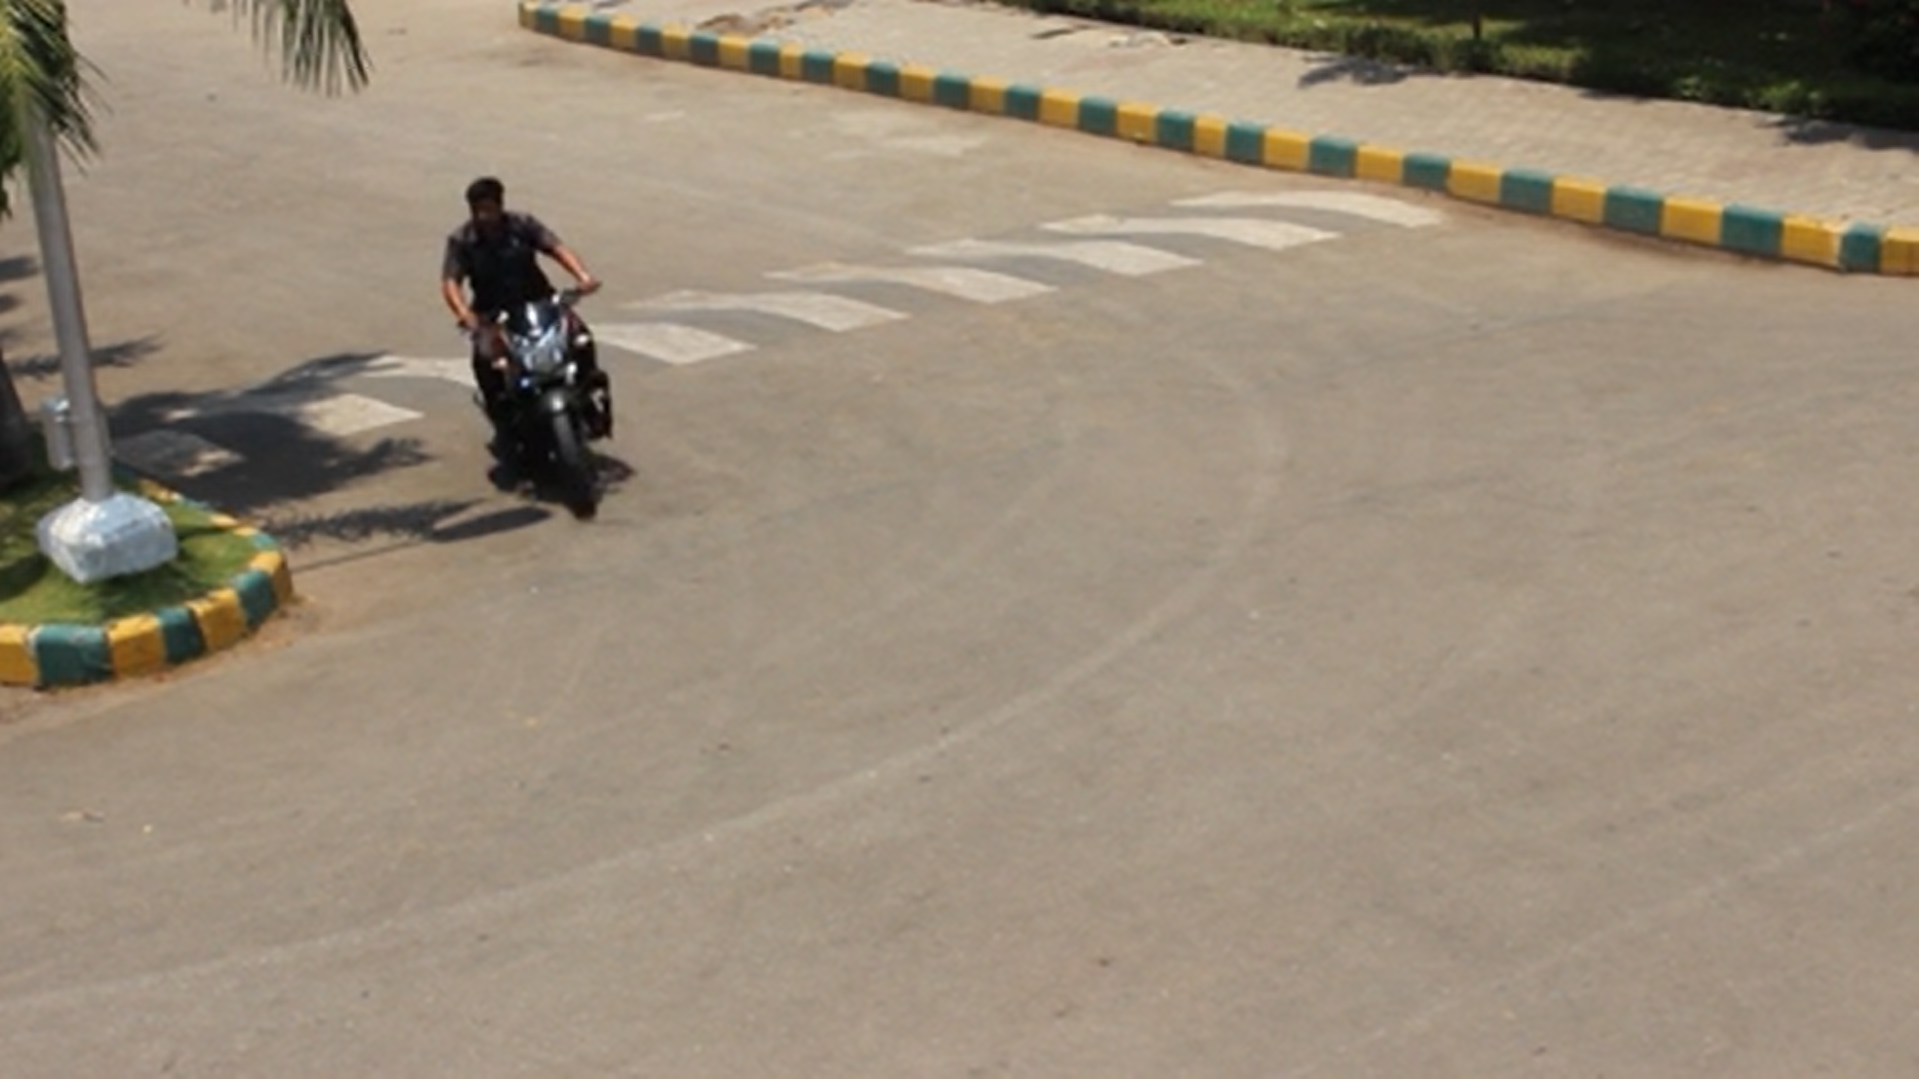
\includegraphics[width=\linewidth]{sample-input-1.png}
    \endminipage\hfill
    \minipage{0.32\textwidth}
        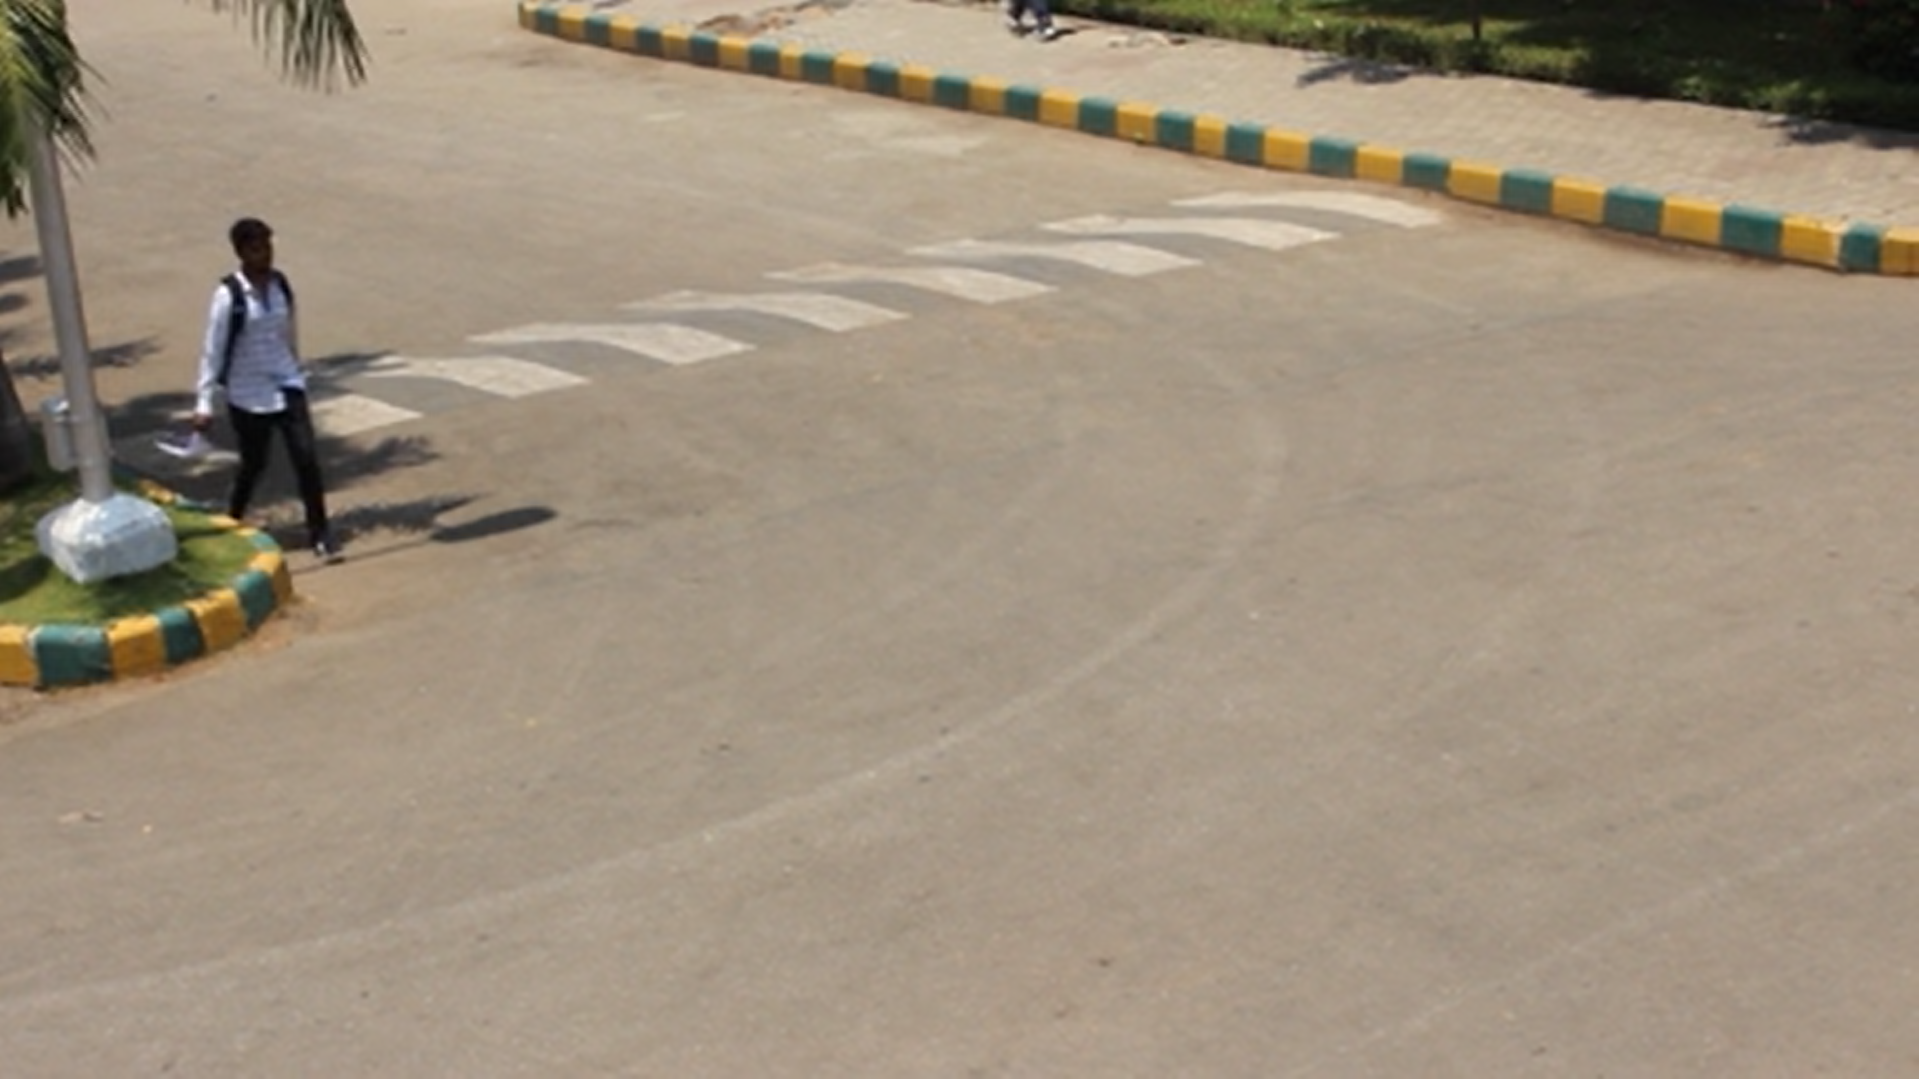
\includegraphics[width=\linewidth]{sample-input-2.png}
    \endminipage\hfill
    \minipage{0.32\textwidth}
        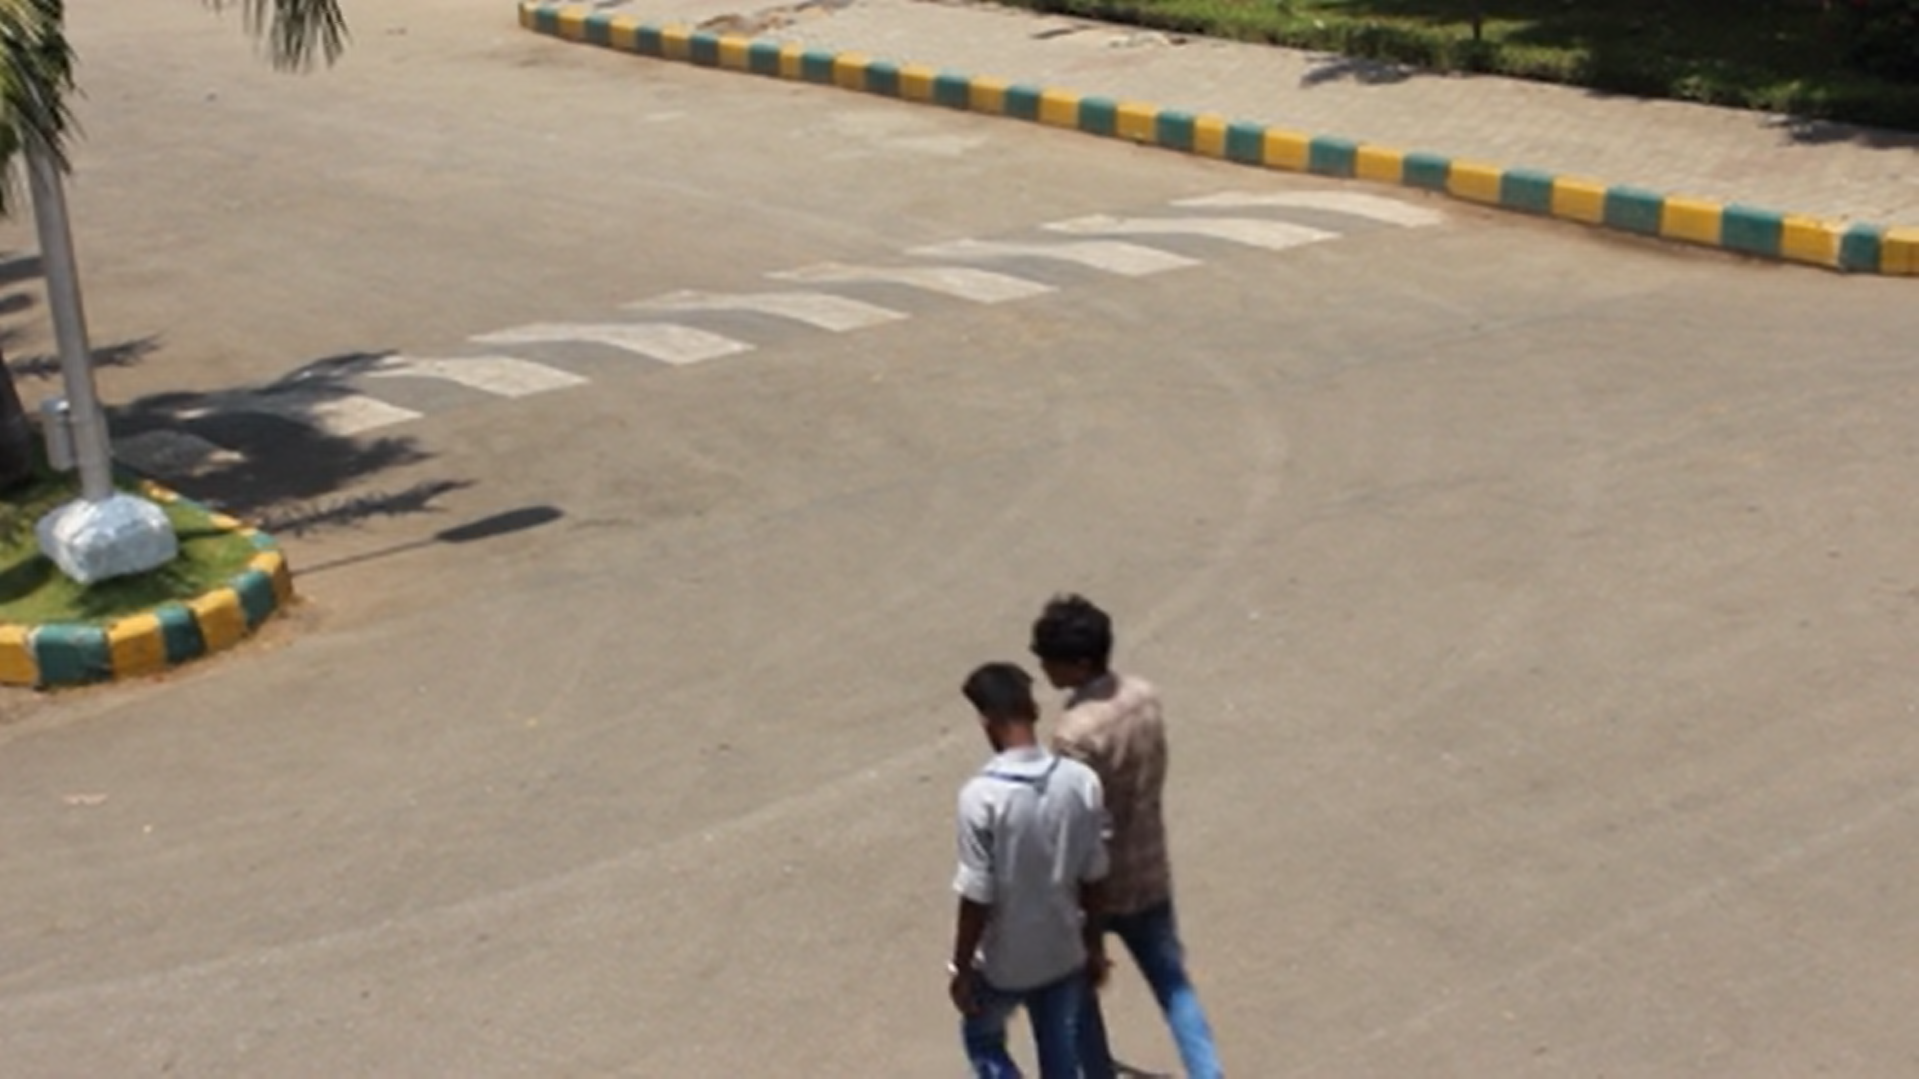
\includegraphics[width=\linewidth]{sample-input-3.png}
    \endminipage
    \caption{Selection of input frames from one of our experimental videos}
    \label{img:sample-input}
\end{figure}

Figure \ref{img:sample-output} shows an output frame generated by our video
summariser. Many people and bikes are seen simultaneously, and the timestamp
shows the time at which the event occurred in the original input video. It is
apparent from this picture that the density of events is dramatically
improved.

\begin{figure}[H]
    \centering
    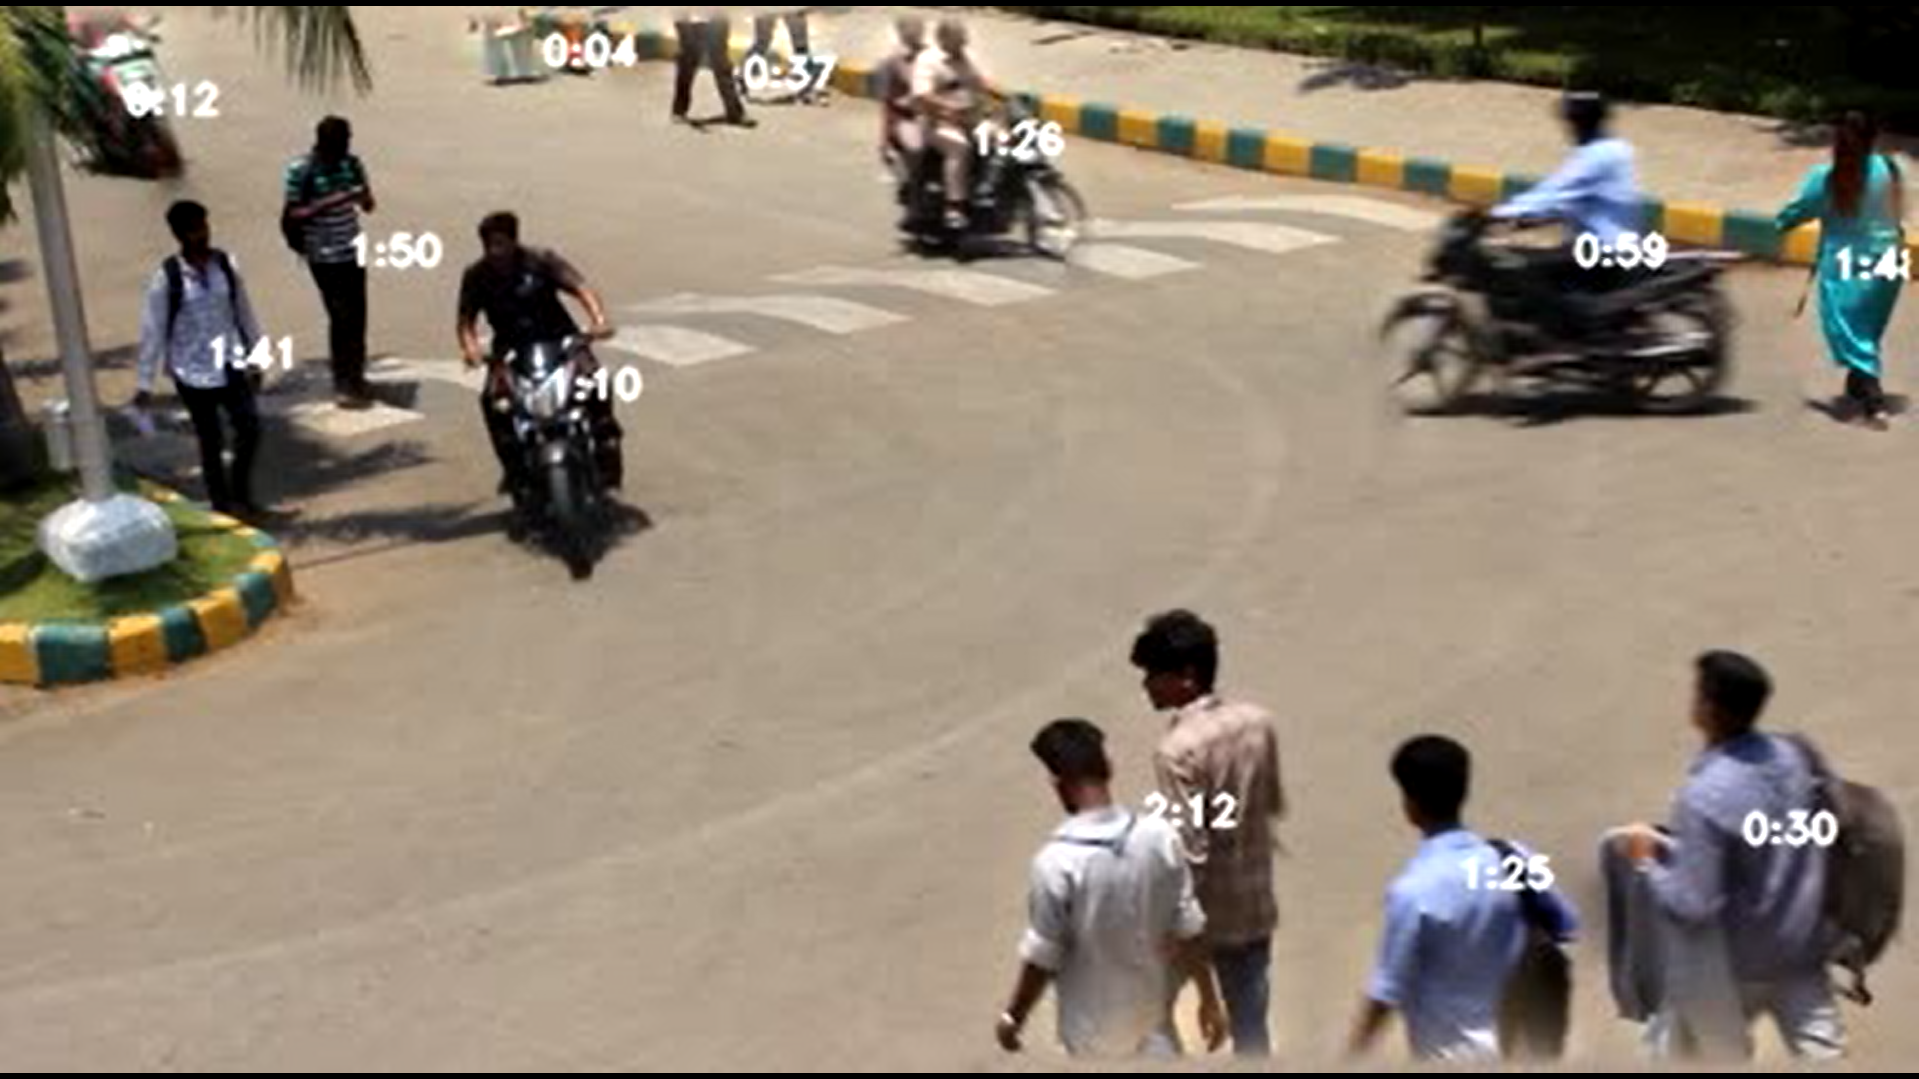
\includegraphics[scale=0.2]{sample-output.png}
    \caption{A frame from the generated summary video}
    \label{img:sample-output}
\end{figure}


\section{Performance Analysis}

This section explains the experimental results of this project. The system
performance was satisfactory and was mostly successful with the tested input
clips, with some limitations which will be mentioned in the further sections.

    \subsection{Objective Evaluation Parameters}

    \begin{itemize}
        \item \textbf{Exhaustiveness of summary}
        The summariser must retain all the events that occurred or the events
        of the specified type in the tag-based summary generation. \\
        Result: All significant events are selected in the events
        \item \textbf{Compression factor}
        Given by Length of original input/Length of summary. The compression
        factor must be as high as possible while keeping the overlap factor to
        a minimum. \\
        Result: There is a compression factor of 4-7x for our sample videos

        \begin{center}
            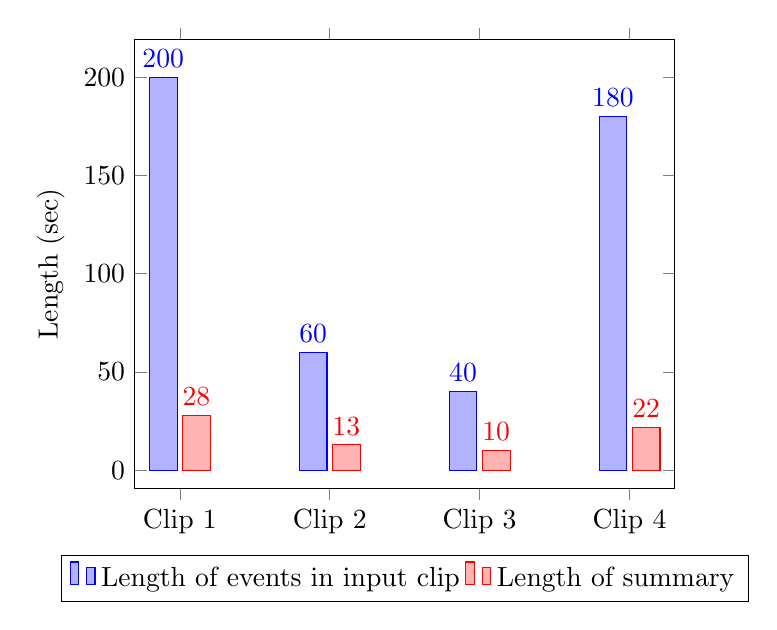
\begin{tikzpicture}
                \begin{axis}[
                    ybar,
                    enlargelimits=0.1,
                    legend style={
                        at={(0.5,-0.15)},
                        anchor=north,legend columns=-1
                    },
                    ylabel={Length (sec)},
                    symbolic x coords={Clip 1, Clip 2, Clip 3, Clip 4},
                    xtick=data,
                    nodes near coords,
                    nodes near coords align={vertical},
                ];
                \addplot coordinates {
                    (Clip 1, 200)
                    (Clip 2, 60)
                    (Clip 3, 40)
                    (Clip 4, 180)
                };
                \addplot coordinates {
                    (Clip 1, 28)
                    (Clip 2, 13)
                    (Clip 3, 10)
                    (Clip 4, 22)
                };
                \legend{Length of events in input clip, Length of summary}

                \end{axis}
            \end{tikzpicture}
        \end{center}


        \item \textbf{Overlap factor}
        A number between 0 and 1 which indicates the amount of overlapping
        (intersection) between the tubes in the summary video. 0 indicates no
        overlap and 1 indicates complete overlap of every clip. \\
        Result: All videos have overlap lower than 0.1
    \end{itemize}

    \subsection{Subjective Evaluation Parameters}

    \begin{itemize}
        \item \textbf{Semantic structure of events}
        Interacting events (that occur in the same time and space) must be
        shown together. \\
        Result: All the interacting events are always shown together
        \item \textbf{Realistic appearance}
        The events must be extracted and be blended into the background
        seamlessly and appear realistic. \\
        Result: Realistic appearance in most cases, with some halo around
        object when at the edges of the frame, or when there is intersection.
    \end{itemize}

    \subsubsection{Performance of Simulated Annealing}
    The simulated annealing optimisation process is not very effective when
    there are a large number of tubes to be re-arranged. The process is
    sensitive to the initial configuration and in some edge cases an optimal
    solution is not obtained. This causes the events in the summary to be
    overlapped. Further improvement in the generation of new configurations and
    an improved cost function will solve the issues faced.

\pagebreak

\section{Summary}

This video summary system which has been developed performs in real-time (30fps)
for the real-time phase and runs reasonably fast in the query phase as well. It
takes about 1 minute for generating a summary video of 10-15 secs.
The outputs are acceptable for the regular summarization (with all events) and
the tag-based summarization, except a few cases where small or fast-moving
objects are not detected. The optimization and blending process can be
improved further to ensure that overlap is further reduced.
